\documentclass[]{report}

\usepackage{pdfpages} 
\usepackage[utf8]{inputenc}
\usepackage[spanish]{babel}
\usepackage{hyperref}
\usepackage{graphicx} % figuras
\usepackage{subfigure} % subfigura
\usepackage{pgfgantt}


% Title Page
\title{Tema de tesis}
\author{Estudiante}



\begin{document}
	
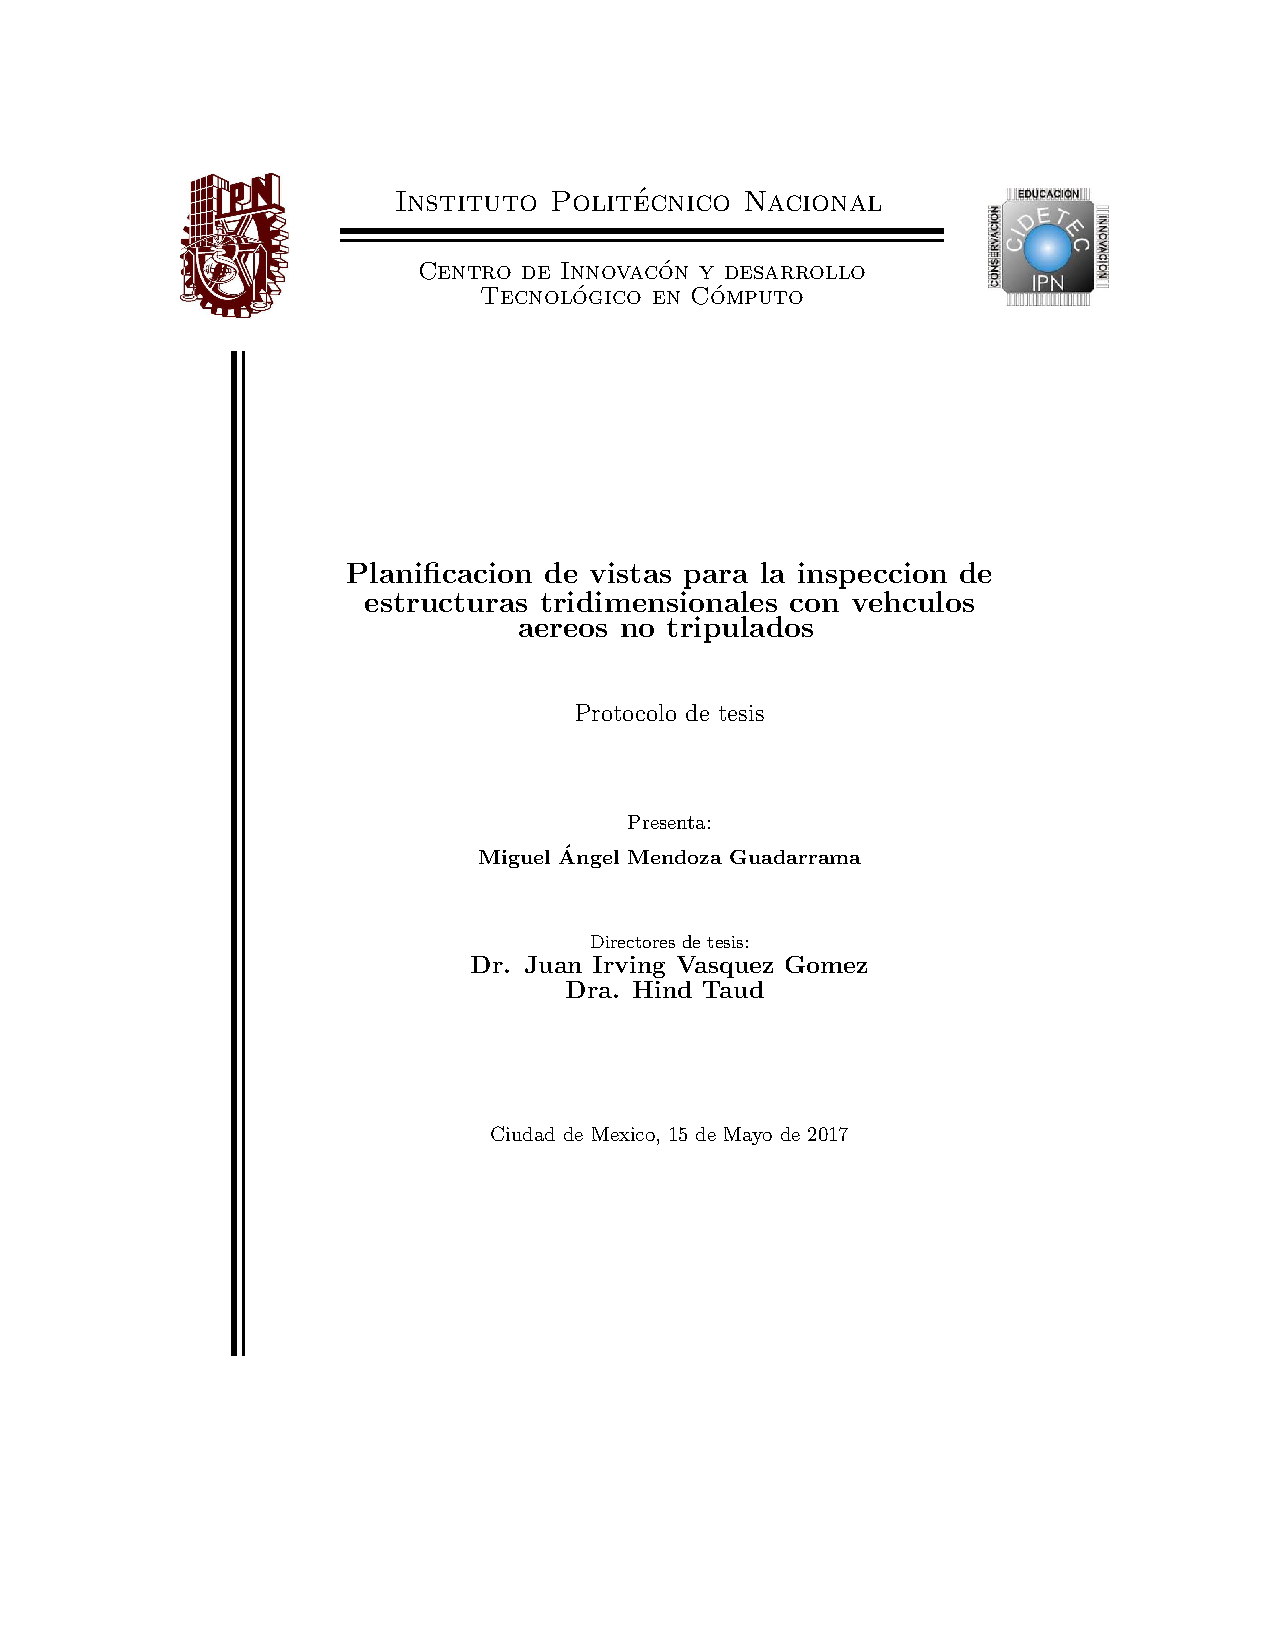
\includepdf[pages={1}]{portada.pdf}
	

\newpage\null\thispagestyle{empty}\newpage
	
%\maketitle

\begin{abstract}
Esta investigación se centra en la automatización de un proceso de inspección visual para contribuir al mantenimiento preventivo, utilizando como herramientas de asistencia: un vehículo aéreo no tripulado (VANT) equipado con un sensor para captar imágenes para tal proceso.
Los avances tecnológicos han contribuido y aportado soluciones valiosas a la humanidad en distintas etapas del tiempo, siempre y cuando  se considere que la tecnología sea empleada como solución a los problemas reales. Entonces surgen una serie de actividades para garantizar la disponibilidad y operabilidad de los dispositivos que nos facilitan las tareas cotidianas recayendo en manteniminetos preventivos. Cuando los mantenimientos preventivos requieren de inversiones altas de tiempo y recursos (dinero, maquinaria, dispositivos, etc) y sobre todo de un alto riesgo humano entonces es cuando las soluciones exigen ser balanceadas para brindar un servicio flexible de acuerdo a las altas exigencias del rápido y continuo crecimiento tecnológico.
Actualmente existen gran cantidad de áreas que requieren de dichas soluciones y en muchas de ellas ya se tienen muchas contribuciones tanto en la parte científica como en la parte industrial usando VANTs equipados con sensores para adquisición de imagenes, como por mencionar algunas: 
i) la industria de la energía eólica, se realizan inspecciones del estado físico de las turbinas de los generadores eólicos para tener una referencia del desgaste sufrido debido a la erosión del contacto con las ráfagas de viento.
ii) Industria de la electricidad: se inspecciona el equipo de transmision de electricidad donde fácilmente pueden ocurrir fallas de suministro por imperfecciones difíciles de detectar debido a su incómodo y peligroso acceso.
iii) en aeronáutica: un robot aéreo toma imágenes del exterior de un avión y se detectan abolladuras con ayuda de supervisión humana, disminuyendo así el tiempo de ejecución actual.
iv) en arquitectura y construcción para evualuación de riesgos y daños: por ejemplo hay aplicaciones dónde se utliza un robot aéreo para  las inspecciones van desde verificar el desgaste y estado en el que se encuentran puentes o presas hasta reconocimiento de fracturas en una construcción después de un lapso de tiempo o inmediatamente después de un temblor.
\end{abstract}

\addtocontents{toc}{\hfill \textbf{Página} \par}
\tableofcontents

\chapter{Introducción}
Un Vehículo Aéreo No Tripulado (VANT) es un robot programado y equipado para volar y ejecutar tareas sin intervención humana. Un VANT ofrece ventajas para tareas que implican escaneos repetitivos de regiones entregando precisión en los resultados, brindan la posibilidad de uso en aplicaciones de alto riesgo o díficil acceso como son: la topografía, mapeado, inspección, monitoreo, agricultura de precisión entre otras. \\
La inspección visual es una técnica que forma parte de los ensayos no destructivos que permite la detección de imperfecciones y defectos en la superficie de un objeto, es importante por que permite predecir futuras fallas potenciales derivadas de superficies defectuosas. La inspección se utiliza en una gran gama de ramas como por ejemplo: en la industria automotriz para soldadura de fabricación y partes de motores; en aviación para verificación del chasis e interiores; en construcción para ensayos de integridad en pilotes y evaluación de riesgos en estructuras; entre muchas otras ramas.
Los Puntos Característicos (PC) en la visión computacional son pequeñas regiones que nos dan información útil de una imagen para distintos propósitos en el área de la visión computacional.\\
\section{Motivación}
Actualmente existen tareas de inspección que requieren el uso de maquinaria de grandes dimensiones, robots de alto costo diseñados para aplicaciones específicas que necesitan de modificaciones significativas para ser usados en otras aplicaiones similares o representan un gran riesgo para el ser humano, entre otras desventajas. En los últimos años, se ha incrementado el uso e interés en VANTs dentro de la comunidad científica y el ámbito industrial para problemas de inspección, principalmente se debe al potencial tecnológico y al gran número de nuevas aplicaciones que brindan.  Dentro de un amplio escenario que permite moverse entre distintas soluciones, para problemas que evolucionan rápidamente, con una flexibilidad razonable dado el rápido avance tecnológico, por lo que su uso se visualiza cada vez más en tareas de la vida real que implican grandes retos tanto de software como de hardware. \\
Automatizar al proceso de inspección para un VANT es más que sólo tomar fotografías desde el cielo, esto implica enfrentar grandes retos como es el proceso de percepción y la planeación de una ruta así como también, cuándo el proceso lo requiera, realizar el procesamiento en tiempo real.
Debido a esto, el uso VANTs capta la atención hacia la visión computacional, la cuál se beneficia de la detección de las regiones mas represetativas de una superficie.
Los PC de un objeto dada su representación digital se convierten en recursos que simplifican los esfuezos para poder medir la cantidad de información útil disponible en imágenes. Esto tiene mucha utilidad para procesos usados en el campo de la visión computacional, ya que amplía el rango de aplicaciones de las cuáles ya se han mencionado algunas y en el ámbito de la inspección ayuda a mejorar su calidad y eficiencia de los resultados obtenidos.
Existen procesos de inspección visual que son de importancia vital como es el de un aeroplano de transporte \cite{sadasivan2005use} dónde muestra que existen varios tipos de entrenamiento para inspección visual y que aproximadamente el noventa porciento de la inspección de un aeroplano es visual. Se han desarrollado simuladores de realidad virtual \cite{sadasivan2005use} y de entrenamiento \cite{gramopadhye2001use} mostrando que es un área que continuamente requiere de inversión de tiempo y recursos computacionales y económicos.\\
En las tareas de inspección de un aeroplano existen tareas repetitivas como menciona Alberts en \cite{alberts1998automated}, tales pueden ser la verificación de la tornillería que fija las cubiertas de aluminio entre otras; entonces si se tiene como asistente un robot que automatice gran parte de las tareas repetitivas ayudará a tener un historial mejor organizado y estructurado para su futura consulta así como también mediciones y herramientas que pueden aportar información valiosa a los fabricantes.\\
Se propone el uso de un VANT equipado con un sensor de adquisición de imágenes y, dado su modelo tridimensional obtener el conjunto de PC para planificar una ruta al VANT que obtenga la covertura total auxilándose de los PC.

\section{Problema}

La automatización del proceso de inspección visual se puede dividir en dos etapas. La primera etapa es el que se va a inspeccionar, es decir la forma en como se va a adquirir la información, la cuál debe de tener un alto grado de autonomía y también debe brindar información de buena calidad y la otra etapa es el cómo se va a analizar ésta información y con qué propósito se utilizará, algunos ejemplos pueden ser en detección de fisuras, mediciones y control dimensional, alineamientos y deformaciones, etc. Este trabajo se centrará completamente en adquirir la información.\\
En el campo de la visión activa, las vistas se refieren a la posición y orientación del sensor en el espacio. Dado un modelo tridimensional, el problema de inspección consiste en determinar las vistas del sensor (de tal forma que se observe por completo el modelo de referencia) y planificar una ruta para inspeccionar el modelo observado. El proceso de inspección, a la entrada requiere de un modelo tridimensional del objeto en cuestión.

\section{Marco Teórico}
Los PC son ubicaciones específicas de una imagen que son mas probables a coincidir en otras imágenes así como también son parte vital en aplicaciones de extracción y detección de características y en técnicas de emparejamiento y rastreo. De acuerdo a \cite{szeliski2010computer} los PC se usan a menudo como precursor a la pose de una cámara y se puede dividir en dos enfoques la búsqueda y correspondencia de PC: una es haciendo una búsqueda local en imágenes tomadas desde puntos cercanos o en sucesiones rápidas y el segundo enfoque es para aquellas aplicaciones donde se esperan muchos cambios de movimiento y posición. Un PC es bueno si: es \textit{repetible}; que la misma característica sea encontrada en varias imágenes sin importar cambios geométricos o transformaciones fotométricas, \textit{saliente}; que cada característica tenga una descripción distintiva y \textit{compacta}; se refiere a que existan menos PC que los pixeles de la imagen.\\
En la imagen \ref{fig:parches} se muestran tres parches extraídos a una imagen: el primero de ellos es una parche sin textura o uniforme lo cuál lo define como un parche difícil de localizar en otras imágenes, el parche central presenta cambios de contraste y, a diferencia del primero es más fácil de localizar en otras imágenes pero debido a que el cambio de contraste sigue casi una línea recta es más difícil de localizar que el tercer parche, el cuál tiene cambios significativos en el menos dos orientaciones distintas. \\

\begin{figure}[h]
\centering
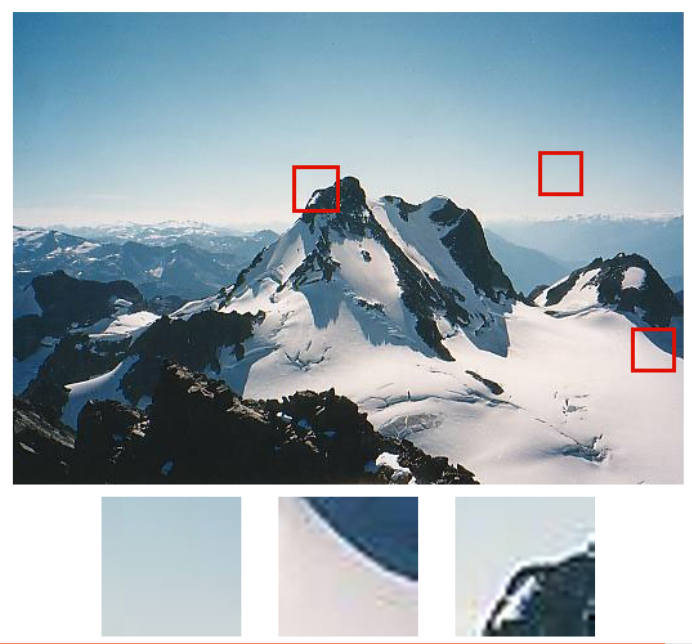
\includegraphics[scale = 0.5]{parches.png}
\caption{Imagen extraída de \cite{szeliski2010computer} dónde muestra tres parches extraídos de una imagen}
\label{fig:parches}
\end{figure}

Existen diversos algoritmos para detectar PC en una imagen como son: esquinas de Harris, SIFT, SURF, ORB, entre muchos otros. Las esquinas de Harris es un detector de regiones en una imagen con altas variaciones en intensidad en todas las direcciones, que básicamente encuentra diferencias en desplazamientos de \textit{x} y \textit{y} en todas las direcciones, un inconveniente del algoritmo de Harris es que tiene un procesamiento muy lento para ser implementado en tiempo real. SIFT (Scale-Invariant Feature Transform) es un algoritmo que permite obtener repetibilidad de PC en distintas imágenes aún cuando hay cambios de escalamiento, el algortimo usa diferencias de Guassianas obtenidas como la diferencia de un difuminado Gaussiano de una imagen con dos valores distintos para $\sigma$. Por ejemplo, un pixel es comparado con sus ocho vecinos así como también con los nueve pixeles en la siguiente escala y también con los nueve pixeles de la escala anterior. SURF (Speeded-Up Robust Features) utiliza filtros de caja para encontrar PC en diferentes escalas y al igual que SIFT es un algoritmo que encuentra puntos aún cuando hay cambios de orientación.\\
SIFT y SURF son algoritmos patentados, es decir que se tiene que pagar para poder implementarlos a diferencia de ORB (Oriented FAST and Rotated BRIEF) que surge como una alternativa a éstos algoritmos (tal y como el nombre del artículo publicado lo indica).  ORB utiliza el algoritmo FAST para encontrar PC y después aplica esquinas de Harris para definir los mejores N puntos de todos los encontrados, para encontrar PC en multi escalas se usan pirámides. Debido a que el algoritmo FAST no calcula orientación, ORB utiliza el método de descriptores BRIEF con modificaciones para obtener un mejor funcionamiento ante rotaciones.


\chapter{Trabajo Relacionado}
 Chang-an Liu \cite{liu2014flying} propone una estrategia que consiste en una función (scoring function) que evalua las mejores vistas para la inspección de un equipo de transmisión de electricidad teniendo como entrada la lectura del modelo 3D. Dicha función está compuesta de tres factores: cantidad de la visión, calidad de la visión y visibilidad, y elige la función que tenga el valor más alto para un conjunto de vistas evaluadas.  Dado el modelo 3D genera candidatos de puntos de vista y sobre cada uno de éstos se evalúa la función para después seleccionar los que obtuvieron los resultados mas altos. La evaluación de ésta propuesta se realiza mediante un experimento, dónde se lleva a cabo una simulación de aisladores caídos (parte a inspeccionar del equipo de transmisión de electricidad) y mencionan que emplean el toolbox OpenGL de Matlab. 


Dentro de los grupos más sólidos que existen en ésta aéra y con contribuciones de código abierto, se encuentra el Laboratorio de Sistemas Autómonos en el Instituto Federal de Tecnología en Suiza:\\
- Kostas Alexis \cite{alexis2017realizing} provee un conjunto de algoritmos propuestos por dicho laboratorio, donde llevan a cabo: \textit{planificación óptima de la inspección}; dónde proponen un algoritmo llamado RRTOT (Rapidly-exploring Random Tree of Trees) que supera las limitantes de conocer primeramente el conjunto mínimo de vistas para posteriormente encontrar la ruta más corta para conectar todas estas vistas, dado que no divide el problema, \textit{planificación de inspección de estructura eficiente}; muestrea las vistas de modo que el camino sea corto mientras asegure su cobertura, \textit{planeación de inspección de cobertura uniforme}; es un algoritmo que realiza el cómputo de un conjunto de caras y para cada una de ellas realiza la inspección asegurando la misma distancia y ángulo para encontrar después la ruta óptima entre ellas, \textit{localización y exploración autónoma}; proponen un algoritmo que brinda la capacidad de mapear un ambiente desconocido, y por último \textit {inspección basada en contacto}; donde un conjunto de puntos seleccionados por un usuario de una estructura previamente inspeccionada y reconstruída, son seleccionados  para ser inspeccionados con ayuda de sondas de ultrasonido de contacto.\\\\
Otra de las investigaciones llevadas a cabo para la reconstrucción de un objeto es la propuesta de J. Vasquez \cite{vasquez2014volumetric}. En la cúal propone un algoritmo para reconstruir un objeto usando un robot móvil con estimación de error, se hace una supoción dual de que el robot conoce la posición y las dimensiones de forma aproximada de dicho objeto.  Ataca el problema de la posición de la siguiente mejor vista (NBV) determinando vistas que cumplan con las siguientes cuatro resticciones: \textit{nueva información}, la NBV debe brindar información de superficies desconocidas; \textit{posición}, la siguiente vista debe ser físicamente alcanzable por el robot móvil así como también debe haber suficiente espacio alrededor para garantizar  su desplazamiento.; \textit{restricciones de sensado}, las superficies deben estar dentro campo y profundidad de visión del sensor; \textit{registro}, la siguiente vista debe tener información de la captura pasada de modo que exista información para realizar unión de las vistas. Dichas restricciones las evalúa en una función de utilidad. También menciona otros aspectos deseables que no son completamente necesarios  como: mayor cobertura de área, distancia de navegación, perpendicularidad e incertidumbre espacial. A diferencia de \cite{liu2014flying} dónde el algoritmo se basa en una representación de mallado tridimensional J. Vazquez \cite{vasquez2014volumetric} utiliza una representación de la escena en voxeles para la reconstrucción de las superficies.


\section{Software disponible}
A continuación se enumeran algunos de los recursos de software disponibles para auxiliar el desarrollo de este trabajo.\\\\
\textbf{ROS}\\\\
ROS (Robot Operating System) es una colección de herramientas, librerías, esquemas e implementaciones para desarrollar aplicaciones robustas y de propósito general para robots, debido a que cuenta con plataformas de distintos robots ayuda a controlar sus comportamientos. Es un marco de trabajo de uso libre que fue creado para fomentar el desarrollar colaborativo de software para robots, lo que significa que tiene contribuciones de muchos laboratorios de todo el mundo en las distintas tareas y ambientes que son necesarios en el desempeño de un robot. En la actualidad es ampliamente usado en la comunidad científica y por departamentos de investigación dentro de la industria.\\\\
\textbf{Gazevo}\\\\
Gazevo es otro simulador  de uso libre que provee herrmientas para aplicaciones robóticas, como son: simulación dinámica, gráficos 3d avanzados, modelos de robot precargados, permite correr simulaciones en servidores remotos, entre otras mas. Inicialmente fue parte primaria de las herramientas usadas por la comunidad de ROS.\\\\ 
\textbf{RotorS}\\\\
RotorS es un simulador de MAV (Micro Air Vehicles) desarrollado por el Laboratorio de Sistemas Autónomos del Instituto Federal de Tecnología en Suiza. RotorS es un complemento del simulador Gazebo que provee algunos modelos de multirrotores, sensores, controles y ambientes. Se menciona que no está limitado al uso con los multirrotores que ya dispone, pero queda como trabajo verificar que el uso de los modelos precargados simulen correctamente con otros vehículos.\\\\
\textbf{OctoMap}\\\\
Existe un entorno de trabajo \textit{open source} que incluye librerías para C++ así como también una implementación en \textit{ROS} llamado OctoMap \cite{octomap}, el cuál es una representación jerárquica de datos de una estructura 3D, ofrece la adaptabilidad y flexibilidad de trabajar con etiquetas discretas  o con modelado probabilístico en caso de trabajar con datos obtenidos de sensores con incertidumbre. Armin Hornung en \cite{octomap}  toma en cuenta tres características útiles para el modelado de la representación de un ambiente: \textit{representación probabilística}, la cuál permite trabajar y unir datos con incertidumbre así como mezclar mediciones de varios sensores, ésta representación menciona que es útil cuando se trabaja en ambientes con obstáculos y se tienen mediciones con ruido; \textit{modelado en áreas desconocidas}, es necesario tener conocimiento de áreas sin asignar para planeación de rutas en caso de exploración y mantiene una \textit{eficiencia} de memoria acorde para la representación del modelo 3D necesario, es decir mantiene ocupada una cantidad de memoria pequeña para largos mapeos. En sus experimentos realizados, obtienen una resolución de 2cm es para un volumen de 7.9 m x 7.3 m x 4.6 m siendo esta la mayor y para un volumen de 292 m x 167 m x 28 m obtienen tres resoluciones: 10, 20 y 80 cm siendo 80cm la menor.\\\\

Los requisitos de sistema no son explícitamente especificados para los simuladores enunciados, debido a que van ligados directamente al tipo de ambiente y el robot  o robots usados en la simulación. Sin embargo hay usuarios que coinciden en usar una configuración de un procesador i7 a 3.3Ghz con 8Gb en RAM y una tarjeta aceleradora de gráficos como mínimo NVIDIA GeForce 210.


\chapter{Propuesta}

Se propone extraer el conjunto de puntos característicos del modelo tridimensional de un objeto para programar la ruta y poses a un VANT,  el cuál debe estar equipado con un sensor para adquirir imágenes del objeto real y entregarlas como información para una inspección posterior.

\section{Hipótesis}
 El uso de puntos característicos en la inspección autónoma mejora la planificación en términos de menos vistas y una mayor probabilidad de localización exitosa.

\section{Objetivo General}
 Diseñar un algortimo que extraiga el conjunto de los puntos característicos de una estructura tridimensional con textura y que determine las vistas de un VANT multirotor para observar dichos puntos.

\section{Objetivos específicos}
Como objetivos específicos para lograr el objetivo general, se enuncian los siguientes:\\
 \textbf {1} Determinar cuáles son los puntos característicos a utilizarse\\
 \textbf {2} Establecer una representación que incorpore la información estructural del objeto y sus puntos característicos.\\
\textbf {3} Diseñar un algortimo que determine las vistas del VANT de tal forma que se cubra la representacion del objeto.\\
\textbf {4} Validar el algortimo en simulación determinando eficacia  y eficiencia\\
\textbf{5} Probar el algoritmo en un VANT real.


\section{Metodología}

Para la identificación de las fases de la metodología se ha planteado el diagrama mostrado en la figura \ref{fig:met}.\\
\textbf{\textit{Modelo 3D de entrada}}: la elección y valoración de un modelo de entrada es importante ya que debemos de tener información adicional extra como es la textura, lo cuál es necesario para demostrar la hipótesis. Se tiene identificado el marco de trabajo OctoMap para la representación estructural del modelo 3D, el cuál se revisará exhaustivamente para determinar si adecuado para ser utilizado como herramienta para éste trabajo.\\
\textbf{\textit{Selección de PC}}: las características que se encuentran en una imagen deben de cumplir ciertas características para que sean considerados como PC, como son: repetibilidad, compactitud y descriptividad. Una vez detectados los mejores PC es posible tener agrupaciones que nos permitan conceptualizar regiones del modelo 3D que van a generar etiquetas fáciles de encontrar.  \\
\textbf{\textit{Localización de vehículo aéreo}}: una vez que se tienen agrupados los PC se procede a generar las vistas del VANT, para ésto es necesario tener generado el modelo cinemático del VANT para ubicarlo en el espacio y planear una ruta de cobertura completa para el modelo a inspeccionar de acuerdo al conjunto de PC.\\
\textbf{\textit{Percepción}}: Se determina la visibilidad del sistema calibrando el sensor de adquisición de imágenes para conocer el campo de visión con el que se puedan percibir los PC,  ésta información es usada para tener infromación de la estructura completa del modelo inspeccionado. Los PC observados en el modelo real se utilizan como información para la estimación de la posición y las imágenes capturadas se presentan como documentación informativa para un proceso de inspección futuro.\\
\textbf{\textit{Validación}}: por último se presenta una validación del desempeño obtenido del algoritmo desarrollado, se proponen que sea evaluado en cuanto a eficacia y eficiencia es decir, porcentaje de cobertura sobre el objeto y tiempo de procesamiento.\\


\begin{figure}[h]
\centering
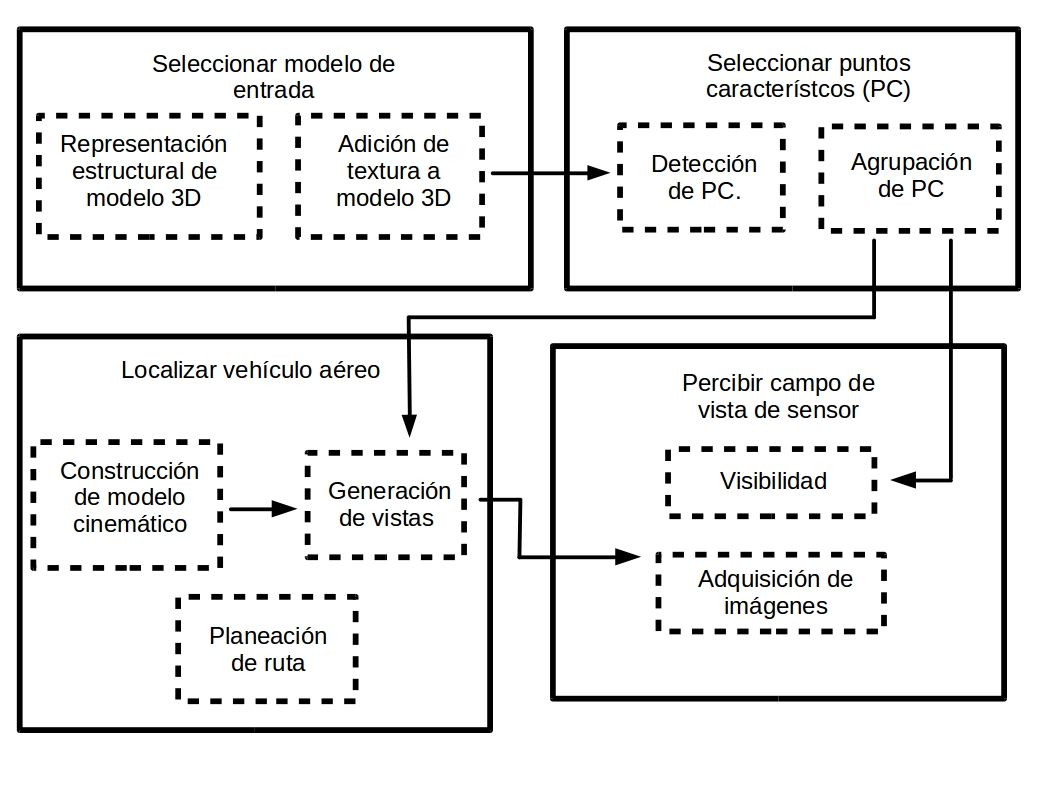
\includegraphics[scale = 0.5]{mapa.jpg}
\caption{Mapa de flujo del método: en cada uno de los cuadros se ilustran las actividades que deben hacer.}
\label{fig:met}
\end{figure}



\subsection{Cronograma}

Se enlistan las tareas que serán ejecutadas durante los semestres 2, 3 y 4 y en la figura \ref {fig:cro}  se muestra su distribución en un diagrama de Gantt.\\\\
1. - Elegir y valorar el modelo a inspeccionar.\\
2. - Valorar e instalar marco de trabajo.\\
3. - Evaluar e implementar algoritmos de extracción de características.\\
4. - Conceptualizar PC\\
5. - Generar modelo cinemático de VANT.\\
6. - Establecer campo de vista del sensor.\\
7. - Enlazar VANT - ROS.\\
8. - Generar vistas del VANT.\\
9. - Generar ruta del VANT.\\
10. - Escribir artículo.\\
11. - Validar de resultados.\\
12. - Presentar de resultados.\\

\begin{figure}[h]
\centering
\begin{ganttchart}[
vgrid,
hgrid,
bar/.append style={fill=blue!100},
]{1}{18}

\gantttitle{Cronograma de actividades}{18} \\
\gantttitle{Semestre 2}{6} \gantttitle {Semestre 3}{6} \gantttitle {Semestre 4}{6} \\
\ganttbar{Tarea 1}{1}{1} \\
\ganttbar{Tarea 2}{1}{3} \\
\ganttbar{Tarea 3}{1}{1}\\
\ganttbar{Tarea 4}{2}{4}\\
\ganttbar{Tarea 5}{3}{6}\\
\ganttbar{Tarea 6}{5}{6}\\
\ganttbar{Tarea 7}{7}{9}\\
\ganttbar{Tarea 8}{7}{8}\\
\ganttbar{Tarea 9}{9}{11}\\
\ganttbar{Tarea 10}{10}{13}\\
\ganttbar{Tarea 11}{13}{16}\\
\ganttbar{Tarea 12}{16}{18}

\end{ganttchart}

\caption{Cronograma de actividades: cada división horizontal representa un mes}
\label{fig:cro}
\end{figure}



\chapter{Avances}

Se presenta la evaluación de los algoritmos ORB y esquinas de Harris  para obtener la eficiencia en cada uno de ellos para una toma efectuada en tiempo real en mismas condiciones.
El procesamiento se realizó usando librerías de OpenCV y se hicieron capturas en tiempo real y despliegue de tiempo de procesamiento para cada algoritmo.\\
Las imágenes obtenidas se muestran en la figura \ref{fig:orb_harris} , donde se muestran los PC encontrados para ORB y para Harris .  Se realizaron cuatro capturas para cada algoritmo: tres con distintas distancias de la imagen a la cámara con el objetivo de cambiar el escalado y otra captura con la imagen rotada.\\
Se puede observar que para el algoritmo de ORB existen algunos puntos que se siguen reconociendo como característicos aún variando la distancia e incluso se hace una rotación para obsevar si algunos de ellos se mantienen y se encierran con círculos rojos los conjuntos de puntos o puntos aislados que se encuentran mas marcados en las imágenes de cada algoritmo. \\
Se ha tomado el tiempo que toma para cada una de los algoritmos realizar el procesamiento de cada una de las fotografías mostradas. Para ORB se tomaron 170 muestras de tiempo de ejecución obteniendo un promedio de 18.42 ms y para Harris de igual forma se tomaron 170 muestras con un promedio de 11.04ms. Durante las pruebas en tiempo real, las imagenes de salida para Harris no fueron tan fluidas como lo fueron para ORB, se tuvieron lapsos de tiempo en pausa hasta de 7 seg para Harris mientras que ORB demostró un comportamiento contínuo y sin pausas.\\
ORB muestra una cantidad mucho mayor de PC encontrados siendo algo complicado su conteo a simple vista mientras que Harris muestra una cantidad menor de puntos incluso se comprueba que es susceptible al escalado y rotación.   También se puede observar que ORB tiene un mejor comportamiento ante posibles cambios de iluminación como se puede observar; que al ir alejando la libreta, la iluminación cambia y algunos PC siguen siendo detectados.\\





\begin{figure}
\centering
\centering
\subfigure[{\scriptsize ORB 1}]{
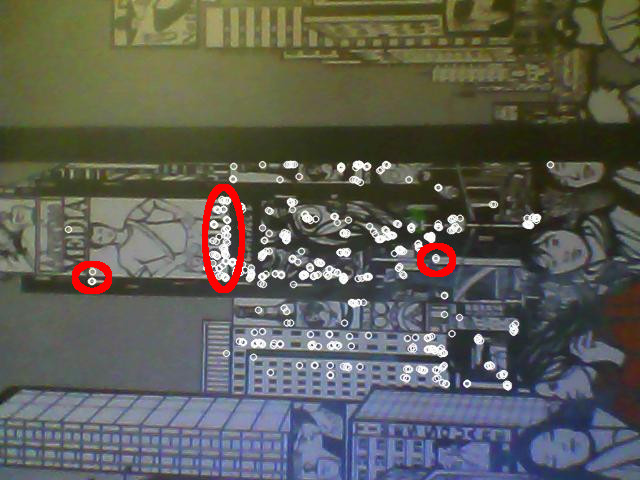
\includegraphics[width=0.42\textwidth]{orb2_b.jpg}

    \label{fig:subfig1}
}
\subfigure[{\scriptsize ORB 2}]{
    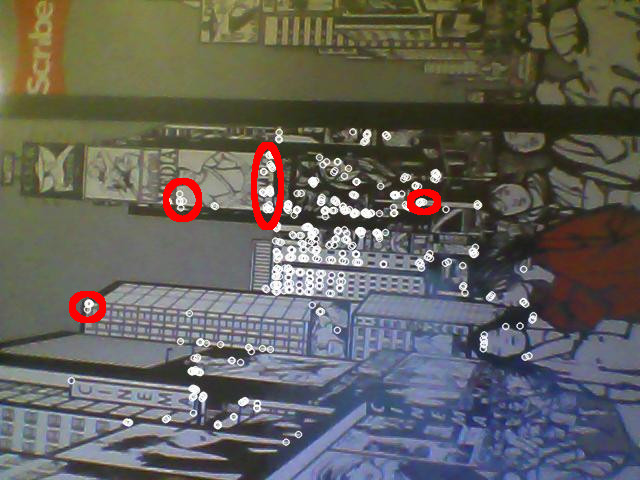
\includegraphics[width=0.42\textwidth]{orb1_b.jpg}
    \label{fig:subfig2}
}
\subfigure[{\scriptsize ORB 3}]{
   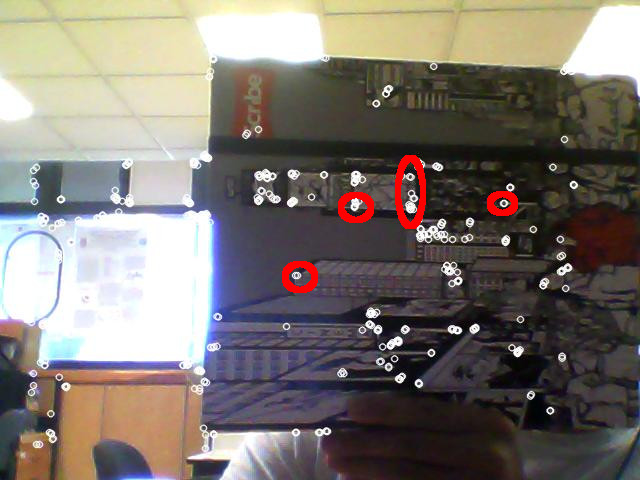
\includegraphics[width=0.42\textwidth]{orb3_b.jpg}
    \label{fig:subfig3}
}
\subfigure[{\scriptsize ORB 4}]{
   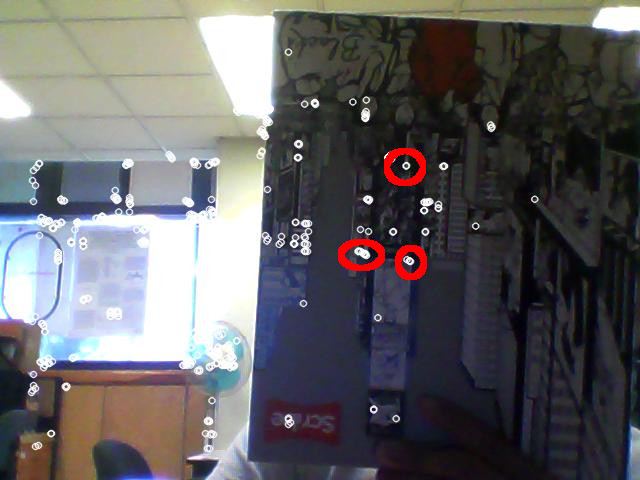
\includegraphics[width=0.42\textwidth]{orb4_b.jpg}
    \label{fig:subfig4}
}

\subfigure[{\scriptsize Harris 1}]{
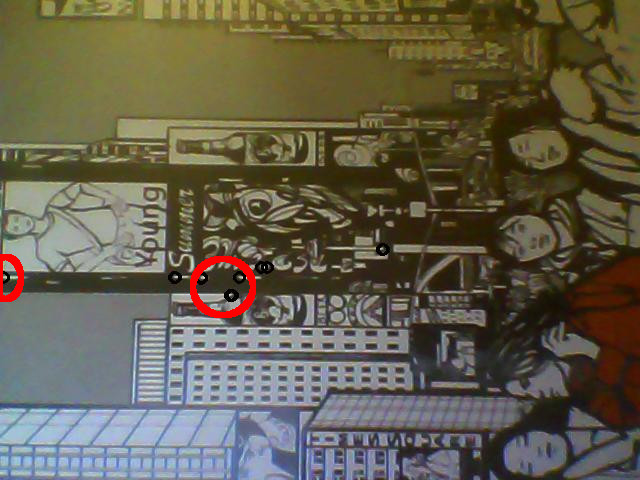
\includegraphics[width=0.42\textwidth]{harris1_b.jpg}

    \label{fig:subfig1}
}
\subfigure[{\scriptsize Harris 2}]{
    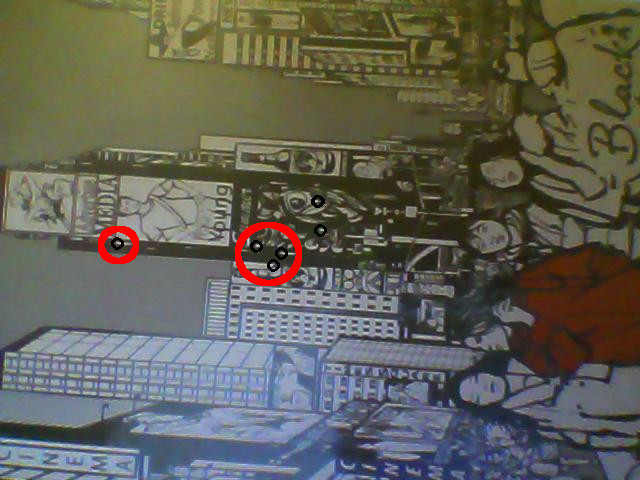
\includegraphics[width=0.42\textwidth]{harris2_b.jpg}
    \label{fig:subfig2}
}
\subfigure[{\scriptsize Harris 3}]{
   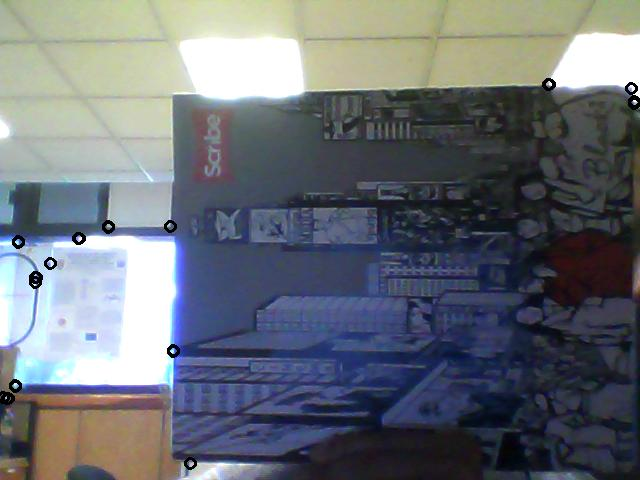
\includegraphics[width=0.42\textwidth]{harris3.jpg}
    \label{fig:subfig3}
}
\subfigure[{\scriptsize Harris 4}]{
   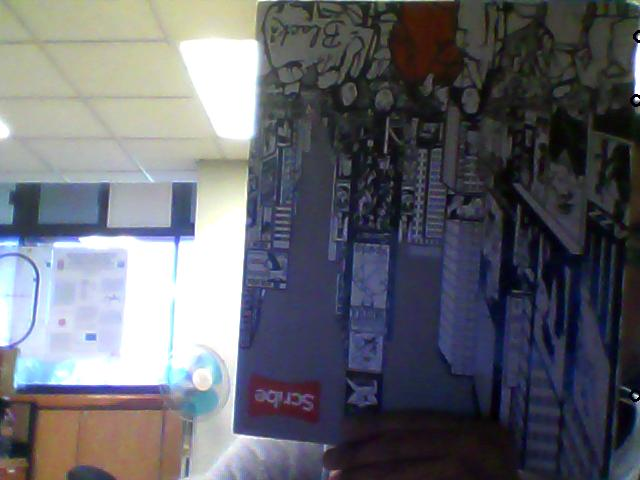
\includegraphics[width=0.42\textwidth]{harris4.jpg}
    \label{fig:subfig4}
}
\caption{Imágenes de la (a) a la (d) muestran los resultados para el agoritmo de ORB mientras que de la (e) a la (h) corresponden a Harris.}
\label{fig:orb_harris}
\end{figure}






\chapter{Conclusiones}

En ésta investigación se aborda el problema de la planificación de ruta a un VANT para realizar inspección a un objeto real partiendo de su representación tridimensional de un objeto.\\ Se propone utilizar los PC del modelo tridimensional con textura como información para planificar una inspección visual usando VANT por lo que agrupando los PC se tiene una descripción de la superficie total.\\
De acuerdo al trabajo mostrado en los avances, la extracción de PC de una imagen usando el algoritmo ORB es mucho más eficiente que el algoritmo de Harris. ORB trabajó correctamente en tiempo real a parte de brindar repetibilidad de los puntos entre variaciones de escala y rotación a difererncia de Harris que presentó pausas hasta de 7 segundos para actualizar resultados entre una toma y otra. Los algoritmos de SIFT y SURF quedan descartados para ser usados ya que al ser patentados se debe pagar por su uso.\\
Se desarrollarán las bases de una herramienta flexible y adaptable para llevar a cabo tareas exhaustivas, repetitivas y en cierto grado peligrosas como los son la inspección de objetos imperativos en tamaño y estructra y que apoyen al ser humano a tomar decisiones. En el área de la visión computacional existen diversos algoritmos que detectan los PC dada una imagen 2d, sin embargo hay pocas aplicaciones específicas que se enfoquen en modelos 3d de grandes dimensiones y arrojen las vistas para que un VANT complemente la planificación de una inspección.\\ Se visualizan problemáticas a enfrentar para complementar ésta tarea, algunas de ellas son la cobertura de zonas difíciles de sensar, reconocer buenos PC pensando que la inspección se puede llevar a cabo en varios modelos, procesamiento de imágenes con ruido e incertidumbre, eficientar tiempo de procesamiento para que el VANT pueda tener capacidad de decisión en caso de existir presencia de objetos no esperados durante la inspeccion y la duración de la batería.

\bibliographystyle{plane}
\bibliography{protocolo}

\end{document} 